\documentclass[12pt,a4paper]{article}
\usepackage{times}
\usepackage{mathptmx}
\usepackage{setspace}
\usepackage[utf8]{inputenc}
\usepackage[french]{babel}
\usepackage[T1]{fontenc}
\usepackage{amsmath}
\usepackage{amsfonts}
\usepackage{amssymb}
\usepackage{makeidx}
\usepackage{graphicx}
\usepackage{lmodern}
\usepackage{index}
%\usepackage{hyperref}
\newcommand{\HRule}{\rule{\linewidth}{0.5mm}}
%\usepackage{kpfonts}
\usepackage{fourier}
\usepackage[left=2cm,right=2.5cm,top=2.5cm,bottom=2.5cm]{geometry}
\author{Sarah Kaddah}
\title{Rapport de stage}

%%%%%%%%%%Interligne
\renewcommand{\baselinestretch}{1.5}
\begin{document}
%%%%%%%%%%%%%%%%%%%%%%%%%%%%%%%%%%%%%%%%%%%%%%%%%%%%%%%%%%%%%%%%%
%%%%%%%%%%%%%%%%%%%%%%1ere page%%%%%%%%%%%%%%%%%%%%%%%%%%%%%%%%%%
%%%%%%%%%%%%%%%%%%%%%%%%%%%%%%%%%%%%%%%%%%%%%%%%%%%%%%%%%%%%%%%%%
%%%%%%%%%%%%%%%%%%%%%%%%%%%%%%%%%%%%%%%%%%%%%%%%%%%%%%%%%%%%%%%%%
\begin{titlepage}
  \begin{sffamily}
  \begin{center}
	\large{Université Paris Diderot - Paris 7 \hfill 2017-2018} \bigskip
	\center{\LARGE{Master 2 Biologie-Informatique/ Bioinformatique}}
	
\begin{tabular}{c}
\\ \\ \\
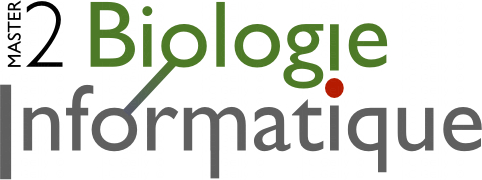
\includegraphics[scale=0.3]{img/m2.png}
\end{tabular}
\hfill
\begin{tabular}{c}
\\

\includegraphics[scale=0.1]{img/p7.png}
\end{tabular}

%%%%%%%%% Title    
    \HRule \\[0.2cm]
    { \huge \bfseries \center{Etude de la fonction et des mécanismes d'évolution des séquences répétées centromériques chez les Primates}\\[0.4cm] }
    \HRule \\%[2cm]
%%%%%%%%Centre de la page    
\begin{center}\LARGE{\textbf{Sarah Kaddah}}\end{center}%~\\[0.1cm]

%%%%%%%%% Bottom of the page
\begin{center}\Large{Tuteur: Lo\"{i}c Ponger}\end{center}~\\%[0.5cm]
\center{\large{Structure et Instabilité des Génomes}}
\center{\large{ MNHN - CNRS UMR 7196 / INSERM U1154 - Sorbonne Universités}}\\%[1cm]
Muséum national d'Histoire naturelle, 43 rue Cuvier 75005 PARIS \\ [1cm]
%	\begin{center}
%		
\includegraphics[scale=0.2]{img/mnhn.jpg} \hfill
%		
\includegraphics[scale=0.08]{img/cnrs.png} \hfill
%		
\includegraphics[scale=0.08]{img/inserm.jpg}
%	\end{center} 

\begin{tabular}{cc}
 \hspace*{2.5cm} &  

\includegraphics[scale=0.2]{img/mnhn.jpg}
\end{tabular}
\hfill
\begin{tabular}{c}

\includegraphics[scale=0.08]{img/inserm.jpg}
\end{tabular}
\hfill
\begin{tabular}{cc}

\includegraphics[scale=0.08]{img/cnrs.png} &
\hspace*{2.5cm}
\end{tabular}

%%%%%%%%% END
  \end{center}
  \end{sffamily}
\end{titlepage}
%%%%%%%%%%%%%%%%%%%%%%%%%%%%%%%%%%%%%%%%%%%%%%%%%%%%%%%%%%%%%%%%%%
%%%%%%%%%%%%%%%%%%%%%Remerciements%%%%%%%%%%%%%%%%%%%%%%%%%%%%%%%%
%%%%%%%%%%%%%%%%%%%%%%%%%%%%%%%%%%%%%%%%%%%%%%%%%%%%%%%%%%%%%%%%%%

\section*{\begin{center}Remerciements\end{center}}~\\[0.2cm]
\addcontentsline{toc}{section}{Remerciements}
Merci à Namrod pour toute la partie sur la bibliographie. Retrouvez ses questions FAQ qui ont permis la rédaction de cette partie.\\
\noindent Merci à f-leb, LittleWhite et Metalman pour leurs conseils et la relecture.
\noindent Merci à ced et jacques\_jean pour la correction orthographique et typographique.
\thispagestyle{empty}

%%%%%%%%%%%%%%%%%%%%%%%%%%%%%%%%%%%%%%%%%%%%%%%%%%%%%%%%%%%%%%%%%%
%%%%%%%%%%%%%%%%%%%Table des matières%%%%%%%%%%%%%%%%%%%%%%%%%%%%
%%%%%%%%%%%%%%%%%%%%%%%%%%%%%%%%%%%%%%%%%%%%%%%%%%%%%%%%%%%%%%%%%

\newpage
\tableofcontents
\setcounter{page}{0}
\thispagestyle{empty}
\newpage 
%%%%%%%%%%%%%%%%%%%%%%%%%%%%%%%%%%%%%%%%%%%%%%%%%%%%%%%%%%%%%%%%
%%%%%%%%%%%%%%%%%%%%Introduction%%%%%%%%%%%%%%%%%%%%%%%%%%%%%%%%
%%%%%%%%%%%%%%%%%%%%%%%%%%%%%%%%%%%%%%%%%%%%%%%%%%%%%%%%%%%%%%%% 

\section{Introduction}
\subsection{Les séquences centromériques}
-> biblio CENP-A\\
-> biblio kinetochore\\
-> info supp sur l'ADN satellite\\

Le centromère est une structure chromatinienne caractérisé par la présence de CENP-A. Cette protéine, très conservée au cours de l'évolution, est un variant de l'histone H3. Son rôle est de fixer la position du kinétochore par un mécanisme encore peu connu. En effet, le centromère est le site d'assemblage du kinétochore, un ensemble d'ADN et de protéines. Il permet l'attachement du fuseau mitotique pour la ségrégation des chromosomes durant la division cellulaire chez les eucaryotes. Le centromère et les protéines impliquées sont relativement bien conservés. Au contraire, l'ADN sous-jacent est très diversifié et l'organisation varie d'un taxon à l'autre. Cependant, une caractéristique commune est retrouvée chez toute les espèces: de l'ADN centromérique répété en tandem nommé ADN satellite. Ces répétitions sont issues d'événements d'amplification, tels les crossovers inégaux, la conversion de gènes, les cercles roulants ou la transposition de séquences.[Malik and Henikoff, 2002; Plohl et al. 2012]
Ces séquences représentent 5\% du génome. Les répétitions s'étendent de 7pb à 3,2kb avec des séquences de 145-180kb le plus souvent.  

\subsection{L'ADN $\alpha$-satellites}
-> première mise en évidence des AS\\
->théorie gradient de l'âge\\
-> travaux sur le gorille à dev\\

L'ADN satellite chez les Primates est connu sous le nom d'$\alpha$-satellite. Ces séquences centromériques répétées en tandem sont riches en AT. 
-> article sur la première découverte

Des études chez l'Homme propose un modèle évolutif. La répartition des $\alpha$-satellites suivrait une répartition spécifique selon l'âge des familles. Les familles les plus jeunes s'insèrent au cœur du centromère, repoussant les familles les plus anciennes jusqu'aux regions voisines, appelé péri-centromère.\\
->Article Shepelev\\
->Est-ce que je peux utiliser du conditionnel? OU est-ce que cette théorie est confirmée?

Un monomère a une longueur de 171pb et il peut être répété des milliers de fois. Les monomères peuvent être répartis en famille selon leur similarité, les séquences ayant un taux d'identité supérieur à 70\%. Ces séquences ont soit une organisation monomérique soit une organisation en répétition d'ordre supérieur (Fig. 1). Dans le premier cas, les séquences d'une même famille sont répétés en tandem. Dans le deuxème cas, une suite de monomères appartenant à différentes familles forme une unité, qui elle est répétée en tandem. 



Ces séquences peuvent avoir un site de liaison à la protéine centromérique CENP-B un motif spécifique de 17pb. Cette protéine, qui reconnaît et se fixe sur l'ADN, serait présente chez de nombreuses familles de Primates. La protéine pJ$\alpha$, une protéine peu caractérisée, reconnaît un motif qui remplace celui de CENP-B.

Les $\alpha$-satellites ont essentiellement été étudiées chez l'homme. Modèle évolutif avec les centromères en expansion. Une hypothèse concernant l'âge des séquences découle de ces recherches: les séquences les plus récentes apparaissent au coeur du centromères, déplançant les plus anciennes au péricentromère. D'autres études chez le gorille ont été faites. Le rôle des $\alpha$-satellites est encore mal connu. 

\begin{figure}
	\center
		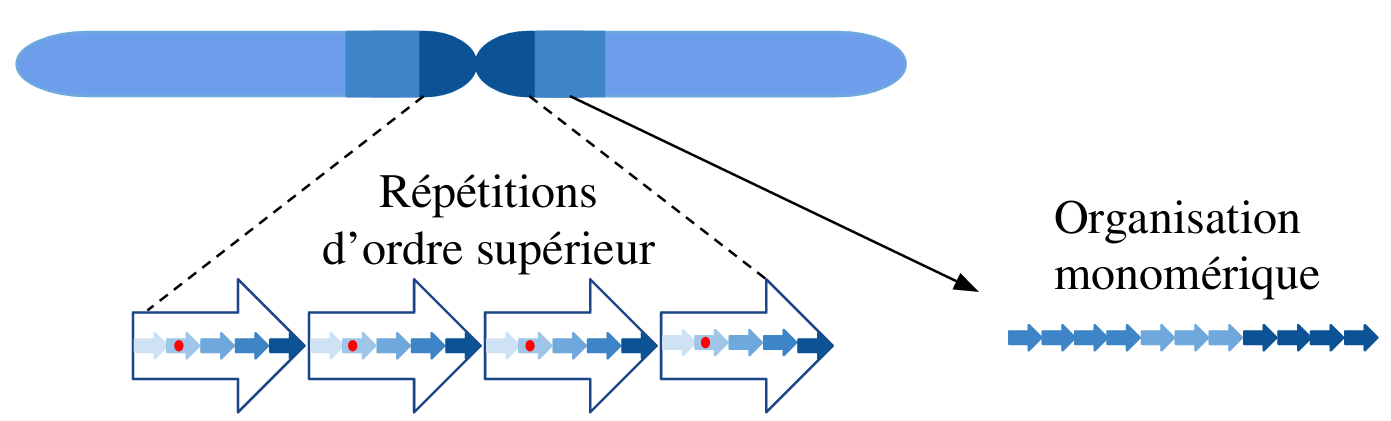
\includegraphics[height=3.5cm, width=12cm]{img/AS_organization.png}
		\caption{\textbf{Organisation spatiale des $\alpha$-satellites:} Le coeur du centromère (bleu foncé) est organisé en répétition d'ordre supérieur. Le péricentromère(bleu clair) a une organisation monomérique. Un monomère d'une même famille est représenté par une petite flèche de même couleur. Les points rouges représentent les sites de fixation à CENP-B ou pJ$\alpha$.}
\end{figure}


\subsection{Le sujet de stage}
enchaîne sur l'étude chez les cerco, une autre étude de séquençage haut débit\\

-travaux précédents limités (expliquer pk). Les méthodes basées aur l'alignement et la phylogénie sont très limitées, le jeu de données étant trop grand. Les méthodes n'étaient pas objectives (quelles méthodes??). De plus, chez d'autres espèces de Primates, les informations sont trop dispersées et aucune comparaison interespèce n'a été faite. \\


L'équipe d'accueil de mon stage "ADN répété, Chromatine, Evolution" ou ARChE, a récemment développé une approche de séquençage haut débit, ciblée sur les séquences $\alpha$-satellites chez deux espèces de Cercopithèques. Une autre étude avec un grand nombre de séquences concerne le Gorille [Catacchio] avec l'utilisation de fragments relativement longs. 

L'objectif de ce stage est de comprendre la fonction des $\alpha$-satellites et leur mécanisme d'évolution. Je vais choisir plusieurs espèces de Primates. Je vais utiliser une méthode de classification automatisée améliorée du laboratoire [Florence Jornod] pour classer les séquences en familles.  Ce programme permet de traiter des centaines de milliers de séquences sans quelque soit le nombre de séquences ou la taille des familles. Je vais dans un premier temps appliquer cette technologies au données issues de ce séquençage. Ensuite, je vais étudier d'autres espèces. Puisque toutes les espèces sont étudiées par la  même méthode, une comparaison inter espèce est envisageable. 

%%%%%%%%%%%%%%%%%%%%%%%%%%%%%%%%%%%%%%%%%%%%%%%%%%%%%%%%%%%%%%%%%
%%%%%%%%%%%%%%%%%%%%%%M & M%%%%%%%%%%%%%%%%%%%%%%%%%%%%%%%%%%%%%%
%%%%%%%%%%%%%%%%%%%%%%%%%%%%%%%%%%%%%%%%%%%%%%%%%%%%%%%%%%%%%%%%% 
\section{Matériel et méthode}
\subsection{Choix des espèces}
	\begin{figure}
		\center
		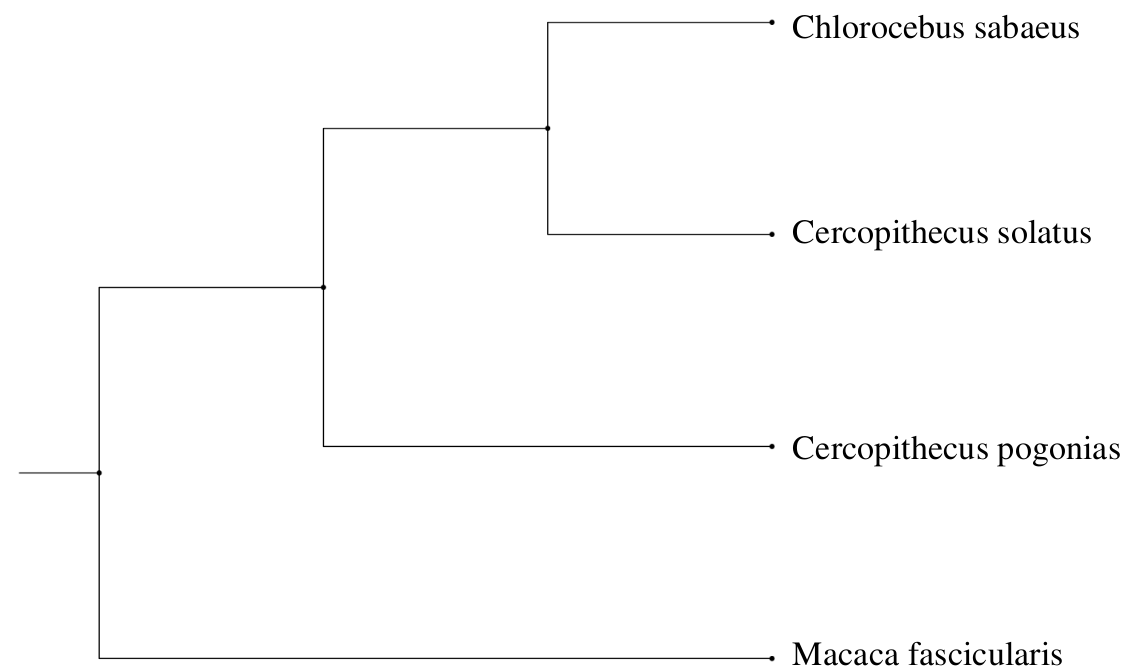
\includegraphics[height=4.5cm, width=7cm]{img/arbre_especes.png}
		\caption{\textbf{Arbre phylogénétique des espèces choisies.}
		\label{fig:arbre_presentation}}
	\end{figure}
Les critères de sélection dépendent de la disponibilité des séquences de qualité. Deux espèces du laboratoire sont choisies, les \textit{Cercopithèques solatus} et \textit{pogonias}, et deux espèces proches (Fig. \ref{fig:arbre_presentation}), le \textit{Macaca fascicularis} et le \textit{Chlorocebus sabaeus}.  

\subsection{Méthode de classification}
	\subsubsection{Principe}
Cette méthode \cite{rapport_florence} répartit des séquences $\alpha$-satellites en familles selon la similarité. La classification est hiérarchique dichotomique. Au départ, une table de 5-mers est calculée pour chaque monomère.  Ensuite, toutes les séquences sont ajoutées dans la file. Ensutie une boucle itérative est exécutée pour séparer les séquences en groupes tant que les nouveaux groupes formés sont divisibles.
	\subsubsection{Répartition itérative}
Une Analyse en Composante Principale (ACP) est effectuée sur la table de fréquence des 5-mers afin de réduire les dimensions du jeu de données et d’obtenir des variables indépendantes. Des distances euclidiennes sont calculées entre toutes les paires de séquence dans l’espace défini par les M premières composantes de l’ACP. A partir du calcul de distance, les séquences sont séparées en deux classes en utilisant la classification hiérarchique basée sur la méthode de Ward. La classification hiérarchique permet de former des classer de façon à maximiser l’inertie interclasse. Cette étape fait un usage important de la mémoire. Par conséquent, pour traiter des jeux de données importants, l’Analyse Discriminante Linéaire , une méthode d’apprentissage, est utilisée sur un sous jeu de données formé par des séquences tirées aléatoirement. Le modèle construit est alors appliqué sur toutes les séquences.
	\subsubsection{Validation d'un sous-groupe}
L'étape suivante est une double validation des sous-groupes. D'une part la taille du sous-groupe est vérifiée. La taille minimale d'une famille est fixée à 100. Si un groupe atteint 100 séquences, il n'est pas redivisé. D'autre part les deux groupes doivent être distincts. Pour cela le \textit{matepair}, la proportion de monomères ayant son plus proche voisin dans le même groupe, est évalué. Des valeurs \textit{matepairs} élevées indiquent des sous-groupes bien homogènes et séparés validant la classification tandis qu’un seuil \textit{matepair} plus faible entraîne plus de classes. Si les \textit{matepairs} sont au-dessus d’un certain seuil, les deux sous-groupes sont ajoutés séparément à la file pour être potentiellement redivisés ultérieurement.En revanche, si au moins une des valeurs de \textit{matepair} est au dessous de ce seuil, les sous-groupes sont considérés comme formant un seul groupe et le groupe initial est sauvegardé comme une famille unique.Si la classification est valide, les deux sous-groupes sont ajoutés dans la file, sinon le groupe initial est sauvegardé comme une classe unique. 

\subsection{Alignement, consensus et phylogénie}
L'alignement des séquence est fait avec muscle \cite{muscle}. La phylogénie est reconstruite avec Seaview 
\cite{seaview} utilisant la méthode du maximum de vraisemblance (PhyML) \cite{phyml}. Le modèle F84 est utilisé pour la construction de l'arbre. Le support de branche est aLRT (SH-like), sans bootstrap. La fréquences d'équilibre nucélotidique est optimisée. Le ratio de transition et transversion est fixé à 4. Aucun site est considéré comme invariable. Le taux de variation à travers le site est optimisé. Les opérations de recherche d'arbre est NNI et l'arbre de départ est défini avec la méthode de Neighbor-Joining \cite{NJ} avec une topologie optimisée.
Les consensus sont obtenus avec des scripts développés par l'équipe. Les motifs CENP-B (TTCGTTGGAA[AG]CGGGA), PJ$\alpha$ (TTCCTTTT[CT]CACC[AG]TAG) et pK$\beta$ (CTATAGGGCCAAAGGAA) ont été identifiés avec le logiciel fuzznuc (package EMBOSS) \cite{emboss} et en autorisant 2 différences au maximum par rapport au consensus. 

%%%%%%%%%%%%%%%%%%%%%%%%%%%%%%%%%%%%%%%%%%%%%%%%%%%%%%%%%%%%%%%%%
%%%%%%%%%%%%%%%%%%%%%%%%%%%%%%%%%%%%%%%%%%%%%%%%%%%%%%%%%%%%%%%%%
%%%%%%%%%%%%%%%%%%%%%%%%%%%%%%%%%%%%%%%%%%%%%%%%%%%%%%%%%%%%%%%%%
\section{Résultat}
	\subsection{Caractérisaton des familles dans plusieurs espèces}
			\subsubsection{Identification des familles}
			Les espèce \textit{C. solatus} et \textit{C. pogonias} sont analysées dans un premier temps pour évaluer la classification automatisée en la comparant avec la classification expérimentale du laboratoire. Expérimentalement, 6 familles $\alpha$-satellites ont été déterminées chez les \textit{Cercopithèques}. Ces deux espèces partagent deux grandes familles monomériques, C1 et C2, de l'ordre de plusieurs milliers de séquences, et deux familles formant un dimère, C3-C4, de l'ordre d'une centaine de séquences chacune. \textit{C. pogonias} possède les familles supplémentaires C5 et C6. Ces familles ont été définies à partir d'une méthode visuelle établie d'après une ACP (Fig. \ref{fig:ACP_exp}).\\
	\begin{figure}	
		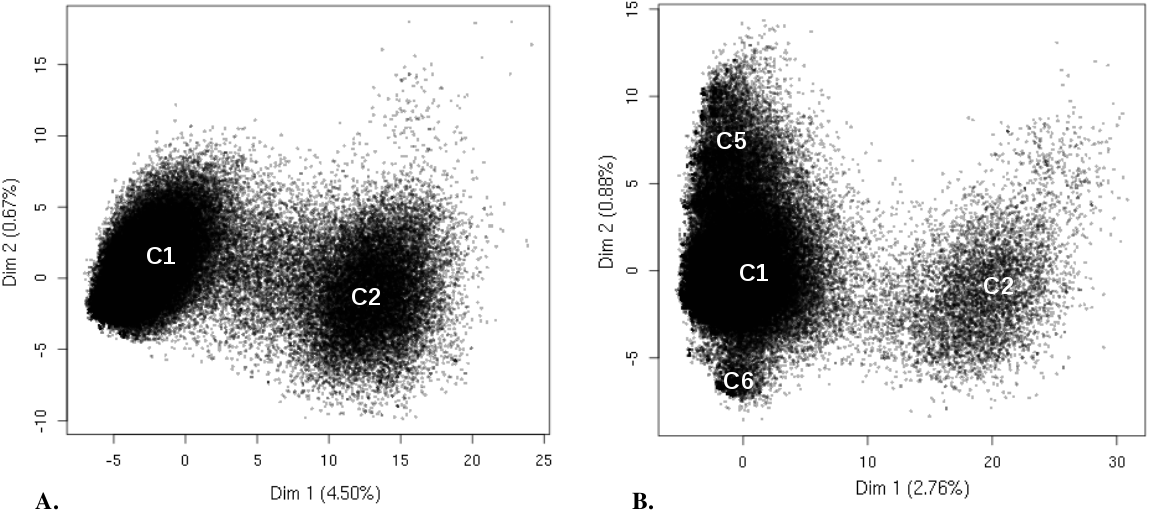
\includegraphics[scale=0.4]{img/ACP_experimental.png}  \\
		\caption{\textbf{Caractérisation visuelle des familles $\alpha$-satellite chez \textit{C. solatus} et \textit{C. pogonias}:}\label{fig:ACP_exp}
		Le nom des familles est indiqué sur les graphiques. Un point représente un monomère. \textbf{A.} Les familles présentes chez \textit{C. solatus}. \textbf{B.} Les familles présentes chez \textit{C. pogonias}.} 
	\end{figure}
	
			La classification automatisée donne des familles de taille variable allant de deux  à des dizaines de milliers de séquences. Seules les familles ayant plus de 100 séquences, appelées "grandes familles", sont conservées pour l'analyse des $\alpha$-satellites. Les "petites familles" sont prises en compte en terme de pourcentage de séquences du jeu de données initial qui ne figurent pas dans l'analyse. Les séquences $\alpha$-satellites chez \textit{solatus} sont réparties en 564 familles, dont 12 grandes familles. Les séquences qui ne sont pas retenues représentent 3,97\% du jeu de données. Chez pogonias, le nombre total de familles est de 132, avec 13 grandes familles et 1,29\% du jeu de données qui  ne figure pas dans les analyses.\\
			
			Bien que le nombre de grandes familles est relativement proche entre ces deux espèces, les résultats expérimentaux diffèrent significativement. Toutes les familles chez \textit{C. solatus} sont retrouvées: 11 familles forment la famille C2, une famille forme la famille C1 et les familles C3 et C4 sont retrouvées dans des petites familles d'environ 80 séquences chacune. Chez \textit{C. pogonias}, toutes les familles sont retrouvées sauf la famille C6. La famille C1 est répartie en 10 familles, les familles C2, C3 et C5 sont retrouvées entièrement, la famille C4 est également retrouvée sous la forme d'une petite famille de 86 séquences. Ces résultats contredisent les résultats expérimentaux. La famille C2 est une famille qui a 85\% d'identité de séquence, comparé à 95\% pour C1. Normalement seule la famille C2 est censée être divisée en plusieurs familles, or ce n'est pas le cas chez \textit{C. pogonias}.
			
\begin{figure}	
	\begin{tabular}{cc|cc}
		  & \textit{C. solatus} &  &  \textit{C. pogonias}\\
		\textbf{A} & 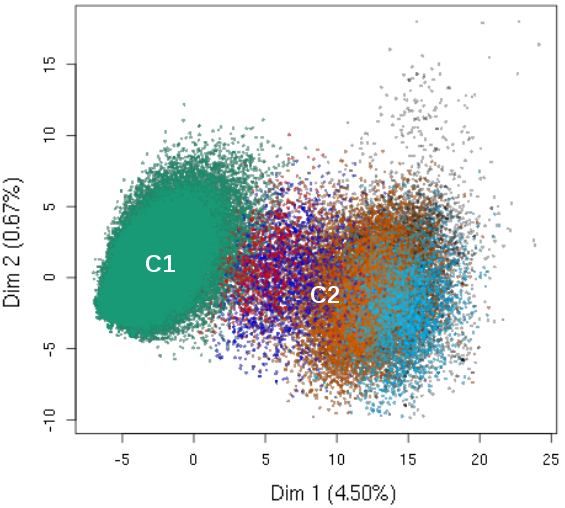
\includegraphics[scale=0.35]{img/solatus_ACP1.png} & \textbf{D} & 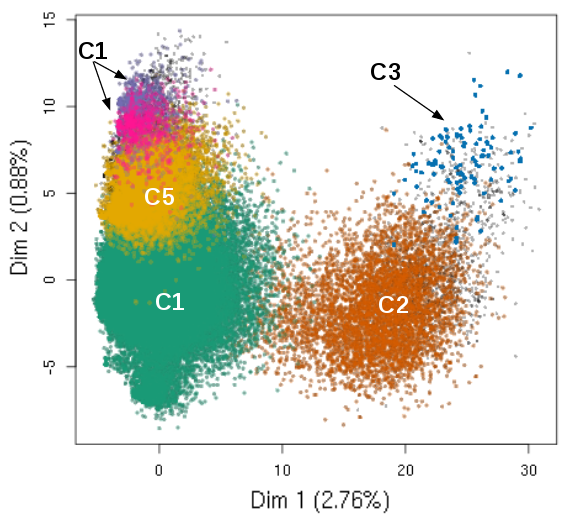
\includegraphics[scale=0.35]{img/pogonias_ACP1.png} \\
		\textbf{B} & 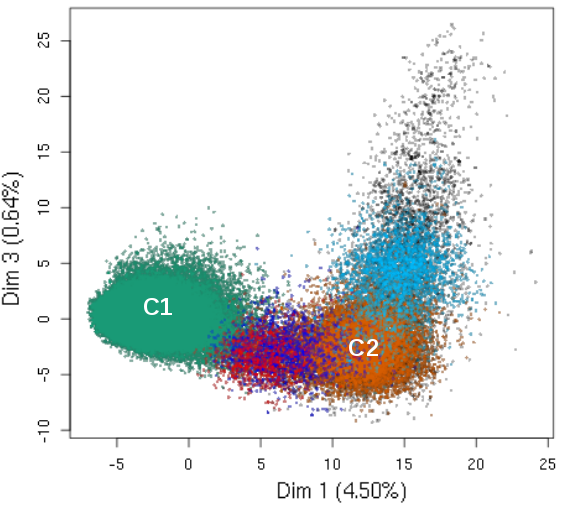
\includegraphics[scale=0.35]{img/solatus_ACP2.png} &  \textbf{E} & 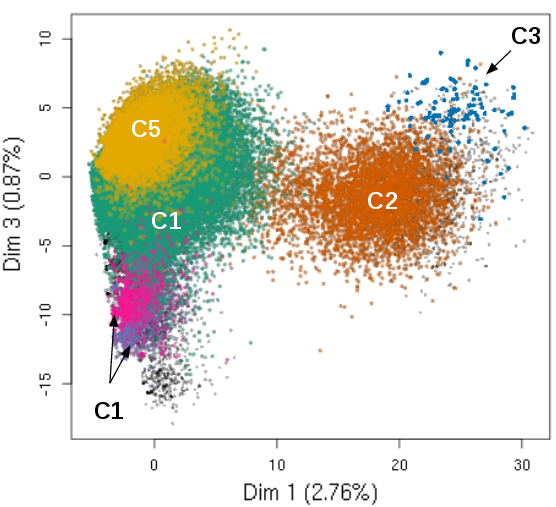
\includegraphics[scale=0.35]{img/pogonias_ACP2.png} \\
		\textbf{C} & 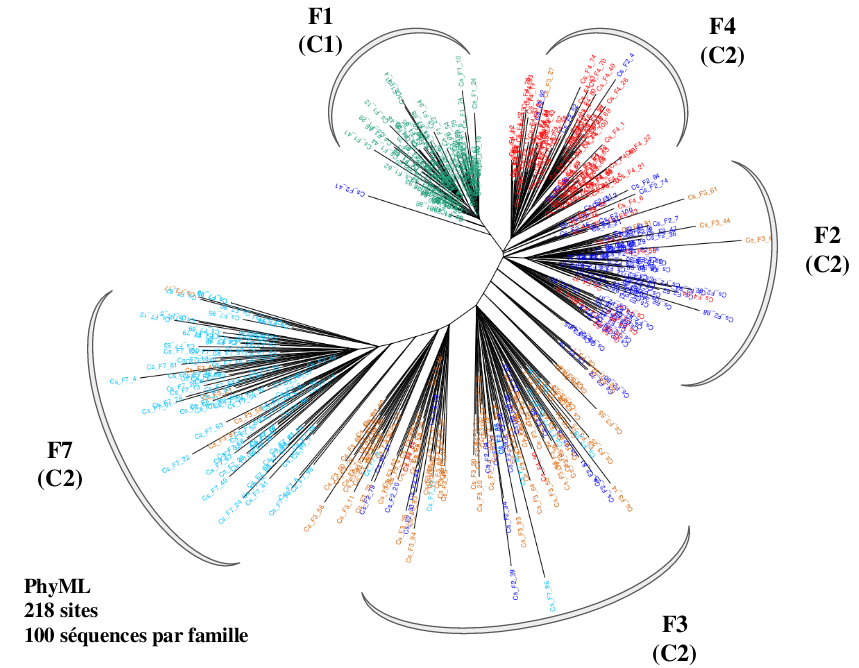
\includegraphics[scale=0.4]{img/tree_solatus.png} & \textbf{F} & 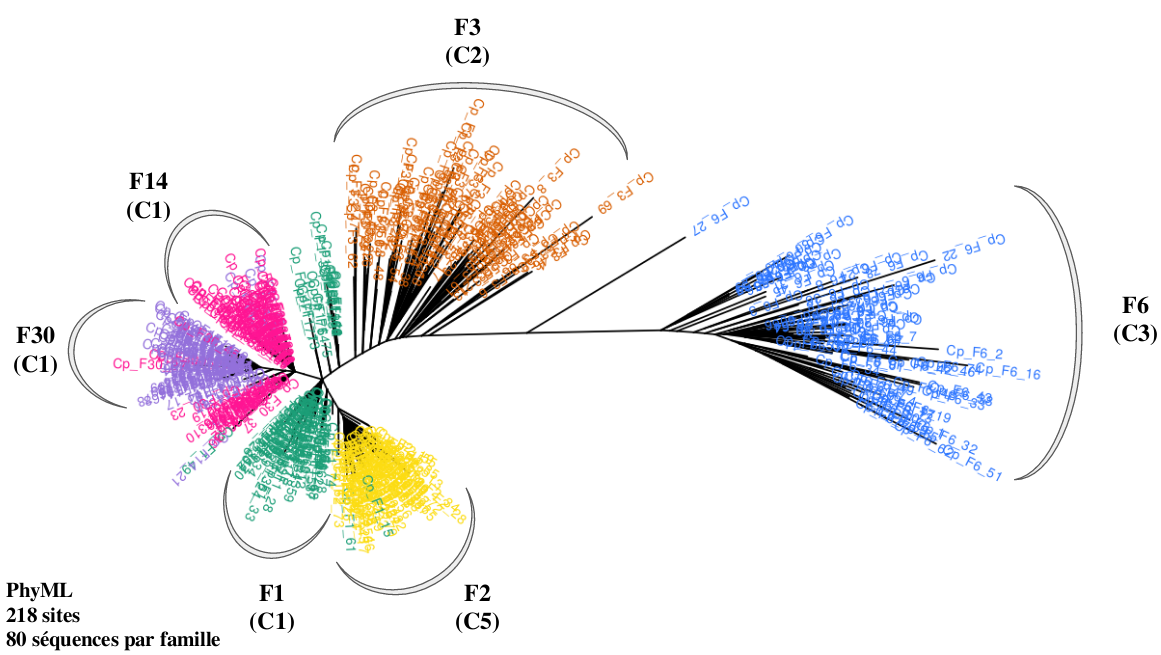
\includegraphics[scale=0.35]{img/tree_pogonias.png} \\
	\end{tabular}
	\caption{\textbf{Les plus grandes familles issues de la classification automatisée:} Les familles expérimentales retrouvées par la classification automatisée sont indiquées sur les représentations de l'ACP des 5-mers.
	\textbf{A.} Composantes 1 et 2 de l'ACP. C1 est en vert, C2 est en orange, rouge, bleu et turquoise.  			\textbf{B.} Composantes 1 et 3 de l'ACP. 
	\textbf{D.} Composantes 1 et 2 de l'ACP. De même pour \textit{C. pogonias}. C1 est en vert, violet et rose, C2 est en orange, C4 est en bleu clair, C5 est en jaune.
	\textbf{E.} Composantes 1 et 3 de l'ACP.
	\textbf{C. et F.} Représentation des familles issues de la classification sous forme d'arbres. Les couleurs des familles sont respectivement conservées et 100 séquences alétoires par familles sont sélectionnées pour la construction de l'arbre. 	 
	\label{fig:so_po_acp_tree}
		} 
\end{figure}
			
			Pour visualiser cette nouvelle répartition des familles, des couleurs sont assignées aux familles issues de la classification automatisée. Ces couleurs sont superposées aux résultats expérimentaux en noir.  Chez \textit{C. solatus}, la famille C1 est entièrement retrouvée. La famille C2 est répartie en plusieurs familles. Deux familles intermédiaires, rouge et bleue, sont visibles entre la famille C1, en vert, et C2, en orange. Elles ne semblent pas distinctes.  Une famille supplémentaire est retrouvée en turquoise, et se démarque. Pour confirmer cette division de la famille C2, la visualisation de l'ACP des 5-mers est observée en fonction des composantes 1 et 3. Les familles intermédiaires restent emmêlées, contrairement à la famille turquoise qui forme une famille à part entière. Pour certifier ce fait, l'arbre construit atteste que chaque famille est bien retrouvée, notamment les familles intermédiaires qui forment bien deux familles. Chez \textit{C. pogonias}, les familles C2, C4 et C5 sont bien retrouvées. La famille C6 se fond dans la famille C1 (en vert). La famille C1 est divisée en deux familles supplémentaires visibles en rose et violet. La visualisation des composantes 1 et 3 de l'ACP ne permet pas de trancher sur la classification. L'arbre montre que les familles C1 en rose et violet sont très proches, et la famille C4 se démarque.  
			 

			 Le \textit{C. sabaeus} a 338 familles au total, dont 44 grandes familles, et 10,89\% du jeu de données qui n'est pas pris en compte. Le \textit{M. fascicularis} a respectivement 709 et 998 familles, dont 42 et 81 grandes familles, et 14,56\% et 5,05\% du jeu de données qui n'est pas pris en compte. Ces espèces ont beaucoup plus de grandes familles que les \textit{Cercopithèques}, et le deuxième jeu de données possède deux fois plus de grandes familles.
			 

			\subsubsection{Motifs CENP-B, pJ$\alpha$ et pK$\beta$}
\begin{figure}	
	\begin{tabular}{cccc} 
		\textbf{A} & 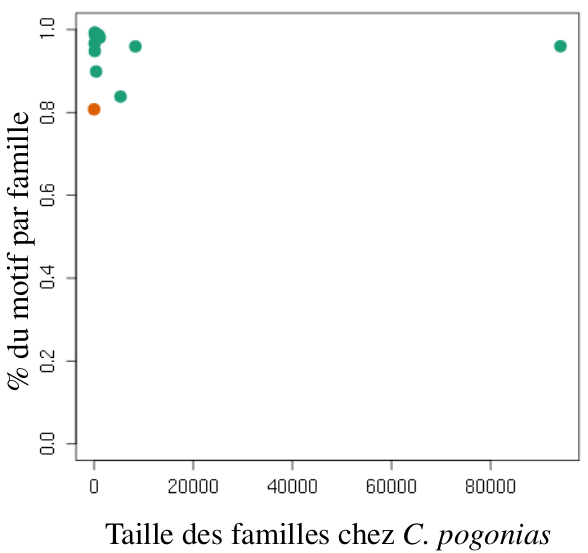
\includegraphics[scale=0.3]{img/motif_pogonias.png} & \textbf{B} 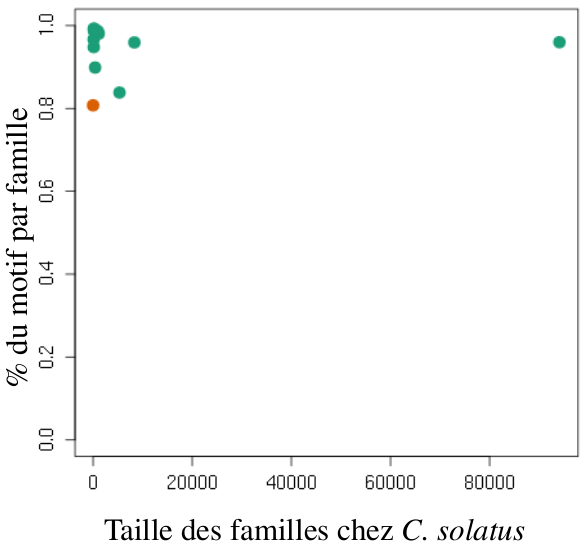
\includegraphics[scale=0.3]{img/motif_solatus.png} \\
		\textbf{C} & 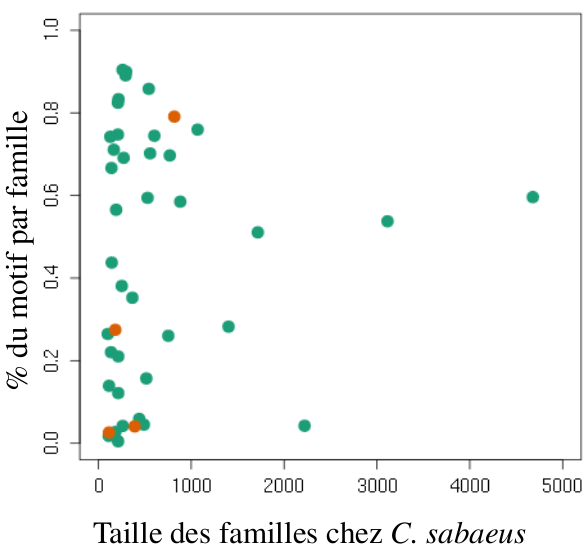
\includegraphics[scale=0.3]{img/motif_sabaeus.png} & \textbf{D} 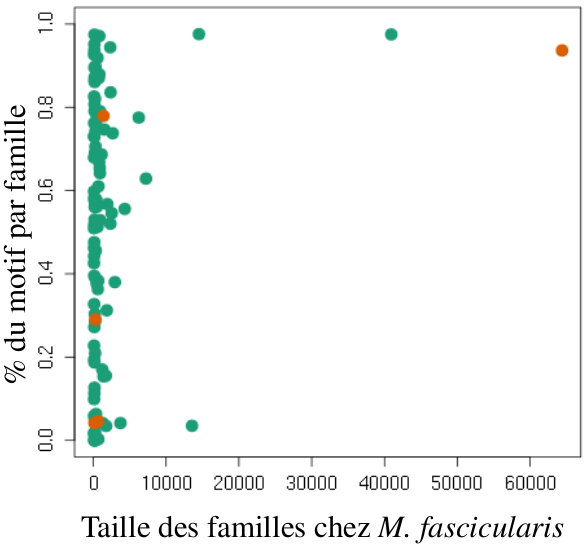
\includegraphics[scale=0.3]{img/motif_fascicularis.png} \\
	\end{tabular}
	\caption{\textbf{Présence des motifs CENP-B, pJ$\alpha$ ou pK$\beta$ par famille:}
	Le pourcentage de séquences par famille ayant le motif pJ$\alpha$ est en vert, pK$\beta$ en orange et CENP-B en bleu. Chaque famille est représentée en fonction de sa taille.
	\label{fig:motif}
		} 
\end{figure}			
			La protéine CENP-B est présente chez toutes les espèces, mais les \textit{Cercopithèques} ne possèdent pas son site de liaison. Cette assertion est vérifiée par l'absence de pourcentage pour ce motif dans les graphes. \textit{C. sabaeus} et \textit{M. fascicularis} n'ont pas ce motif non plus.
			
			Au contraire, la protéine pJ$\alpha$ est très présente chez \textit{C. solatus}, en moyenne a 90\%, et \textit{C. pogonias}, en moyenne à 85\%. La plus grande famille, C1, ayant plus de 80 000 séquences, se démarque avec un pourcentage à  95\%. \textit{C. sabaeus} et \textit{M. fascicularis} ont des pourcentages pour le motif pJ$\alpha$ qui varie entre 1\% et 97\%. Parmi ces familles, \textit{C. sabaeus} a une grande famille de 2 200 séquences qui possède très peu ce motif. Le \textit{M. fascicularis} deux grandes familles, de 20 000 et 40 000 séquences ont ce motif à 97\%. 
			
			Le motif pK$\beta$ est présent lorsque pJ$\alpha$ est absent de la famille. Il est absent chez \textit{C. pogonias}. Une seule famille a ce motif à 80\% chez \textit{C. solatus}, la famille C3,  et chez \textit{C. sabaeus} . \textit{M. fascicularis} a deux grandes familles de plus de 10 000 séquences et plus de 60 000 séquences qui ont respectivement 80\% et 95\% le motif. Ce motif 
			
			Une hypothèse supposerait que les familles ayant un grand pourcentage de pJ$\alpha$ sont des familles apparues récemment. Les familles les plus anciennes auraient accumulé plus de mutations à cet endroit, réduisant ainsi le pourcentage de ce motif.
			
			\subsubsection{Similarité entre familles}
\begin{figure}	
	\begin{tabular}{cccc} 
		\textbf{A} & 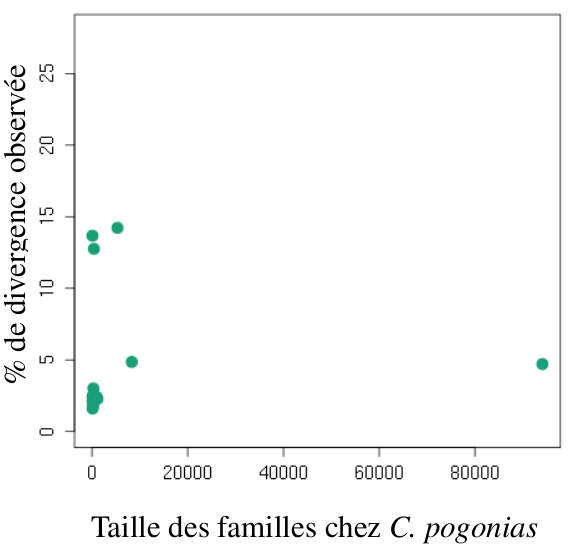
\includegraphics[scale=0.3]{img/similarity_pogonias.png} & \textbf{B} 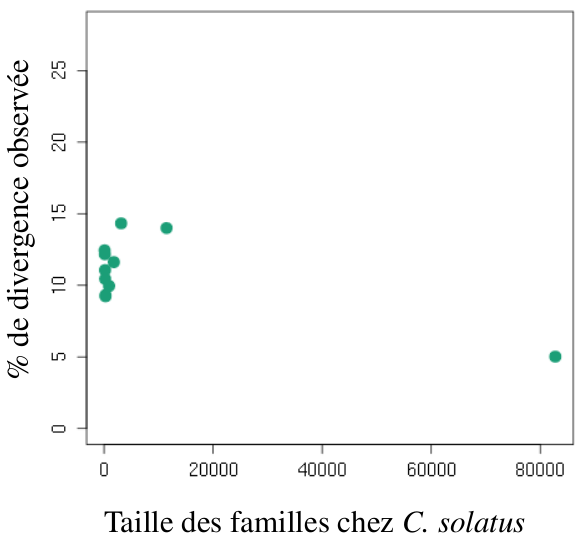
\includegraphics[scale=0.3]{img/similarity_solatus.png} \\
		\textbf{C} & 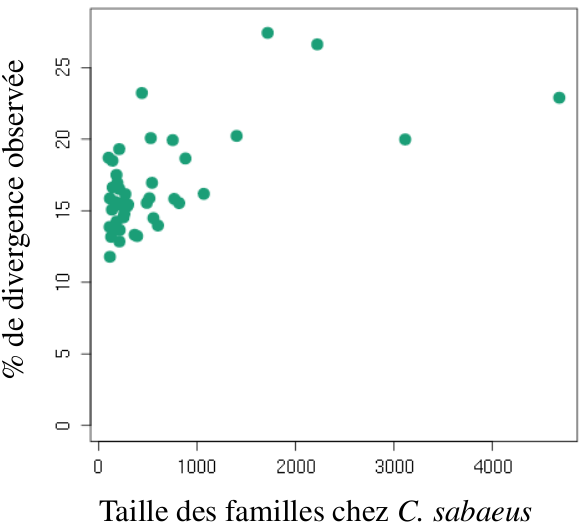
\includegraphics[scale=0.3]{img/similarity_sabaeus.png} & \textbf{D} 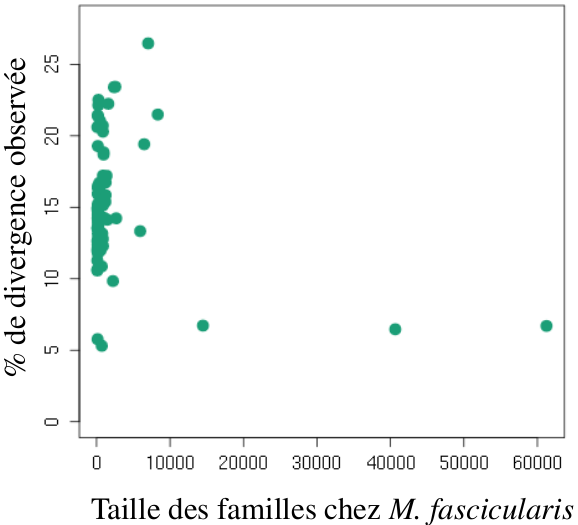
\includegraphics[scale=0.3]{img/similarity_fascicularis.png} \\
	\end{tabular}
	\caption{\textbf{Pourcentage de divergence observée au sein d'une famille:}
	Un point correspond à une famille et représente le pourcentage de divergence en fonction de la taille de la famille.
	\label{fig:motif}
		} 
\end{figure}				
	\textit{C. solatus} et \textit{C. pogonias} ont un pourcentage de divergence qui est relativement faible qui ne dépasse pas les 15\%. La  famille C1 a un pourcentage de divergence très faible de 5\%. Cette grande famille de plus de 80 000 séquences est donc probablement une famille récente.  \textit{C. pogonias} a d'autres familles qui ont un pourcentage en dessous de 5\%.
	\textit{C. sabaeus} a les pourcentages de divergence les plus élevés, allant jusque 28\%, quelque soit la taille de la famille. Cette espèce a des familles anciennes d'$\alpha$-satellites ou alors cette divergence est le résultat d'erreurs de séquençages. Le \textit{M. fascicularis} a des poucentages de divergence qui varient entre 5\% et 27\%. 3 grandes familles ayant plus de 10 000 séquences ont un pourcentage de divergence qui se rapproche de 5\%. Ces familles sont probablement récentes.
	
	\subsection{Comparaison inter-espèce et mécanismes d'évolution}


\section{Discussion}
\section{Conclusion}

\newpage
\strut  ~  \mbox{}  \null
\newpage

\bibliographystyle{unsrt} \bibliography{biblio} 

%
%	\makeindex % index général
%   \newindex{env}{enx}{end}{Environnements}
%   \newindex{ext}{exx}{exd}{Extensions}
%   \newindex{cmm}{cmx}{cmd}{Commandes}
%	\newcommand{\commande}[1]
%   {\texttt{\textbackslash #1}}
%	\newcommand{\indexcmm}[1]
%   {\index[cmm]{#1@\commande{#1}}} % index d'une commande
% 
%
%
%
%Une citation\index{citation} hors paragraphe
%se met dans un environnement
%\emph{quote}\index[env]{quote}
%ou \emph{quotation}\index[env]{quotation}
% 
%L'extension \emph{array}\index[ext]{array}
%fournit les commandes
%\commande{raggedleft}\indexcmm{raggedleft}
%et \commande{raggedright}\indexcmm{raggedright}.
% 
%\printindex % index général
%\printindex[env]
%\printindex[ext]
%\printindex[cmm]

%%%%%%%%%%%%%%%%%%%%%%%%%%%%%%%%%%%%%%%%%%%%%%%%%%%%%%%%%%%%%%%%%%
%%%%%%%%%%%%%%%%%%%%Résumé & Abstract%%%%%%%%%%%%%%%%%%%%%%%%%%%%%
%%%%%%%%%%%%%%%%%%%%%%%%%%%%%%%%%%%%%%%%%%%%%%%%%%%%%%%%%%%%%%%%%%
\newpage 
\thispagestyle{empty}
\section*{Résumé}~\\[0.2cm]
Votre résumé commence ici...
   ...
\section*{Abstract}~\\[0.2cm]
 Abstract begins here...
   ...
\end{document}
%
%%HELP: http://lataix-sebastien.developpez.com/tutoriels/latex/memoire-de-fin-d-etude/#LII-C